\documentclass[border=12pt]{standalone}
\usepackage{amssymb}
\usepackage{amsmath}
\usepackage{tikz}
\usetikzlibrary{arrows.meta, decorations.pathreplacing, calc, positioning, shapes.geometric}

% Project palette (matches covering_diagram_why_curve.tex)
\definecolor{cnavy}{HTML}{0E2747}
\definecolor{corange}{HTML}{E8573F}
\definecolor{cgreen}{HTML}{3B9B6D}
\definecolor{cslate}{HTML}{5B6680}
\definecolor{cmuted}{HTML}{9B9484}
\definecolor{ccream}{HTML}{FAFAF6}

\begin{document}
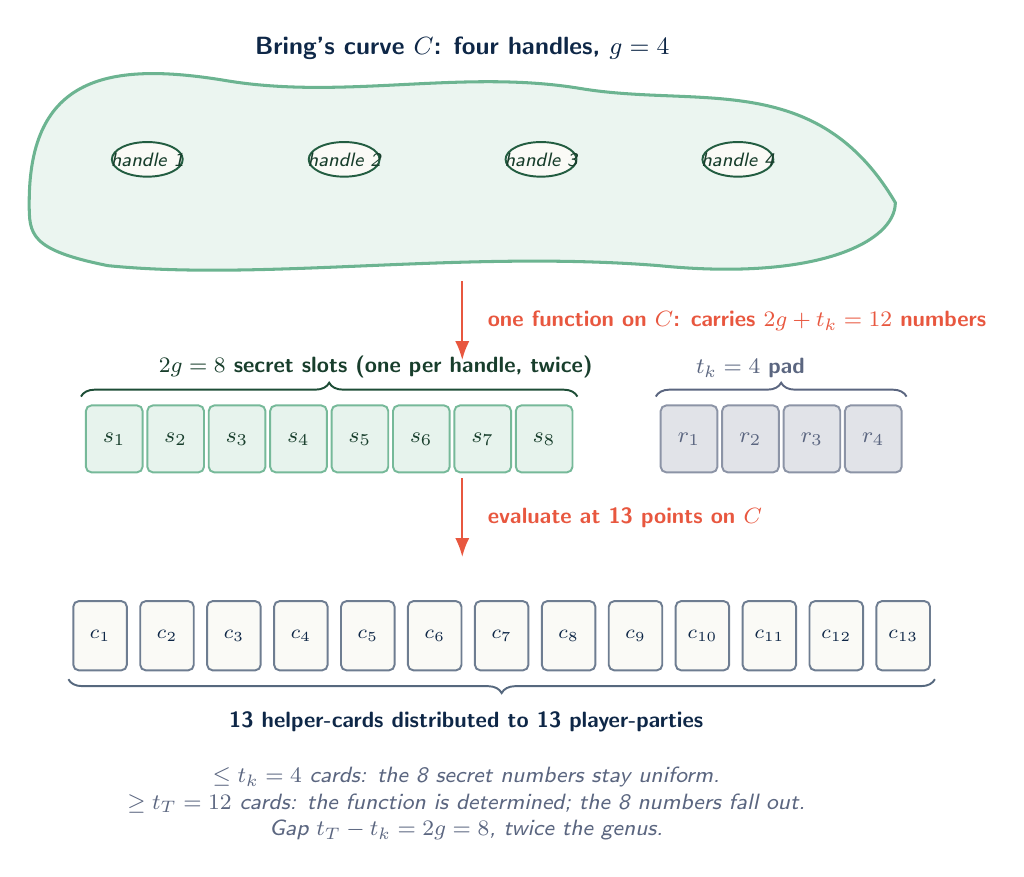
\begin{tikzpicture}[
  secretslot/.style={
    rectangle, rounded corners=2pt, draw=cgreen!70, fill=cgreen!12,
    line width=0.7pt, minimum width=0.72cm, minimum height=0.85cm,
    inner sep=0pt
  },
  padslot/.style={
    rectangle, rounded corners=2pt, draw=cslate!70, fill=cslate!18,
    line width=0.7pt, minimum width=0.72cm, minimum height=0.85cm,
    inner sep=0pt
  },
  helpercard/.style={
    rectangle, rounded corners=2pt, draw=cnavy!60, fill=ccream,
    line width=0.7pt, minimum width=0.68cm, minimum height=0.88cm,
    inner sep=0pt
  },
  flowarrow/.style={
    -{Latex[length=2.4mm]}, draw=cslate!60, line width=0.6pt
  },
  font=\sffamily
]

% ============================================================
% Top band: stylised genus-4 surface (4 handles)
% Surface outline as a rounded blob with 4 inset holes
% ============================================================
\node[cnavy, font=\sffamily\bfseries\small, anchor=south]
  at (8.5, 12.7) {Bring's curve $C$: four handles, $g = 4$};

% Outer surface (smooth-ish closed contour)
\draw[cgreen!75, fill=cgreen!10, line width=1.1pt]
  (3.0, 11.0) .. controls (3.0, 12.6) and (4.0, 12.8) ..
  (5.5, 12.55) .. controls (7.0, 12.3) and (8.5, 12.7) ..
  (10.0, 12.45) .. controls (11.5, 12.2) and (13.0, 12.7) ..
  (14.0, 11.0) .. controls (14.0, 10.5) and (13.0, 10.0) ..
  (11.0, 10.2) .. controls (8.5, 10.4) and (6.0, 10.0) ..
  (4.0, 10.2) .. controls (3.0, 10.4) and (3.0, 10.6) ..
  cycle;

% 4 holes (handles, drawn as small inset ellipses)
\foreach \i/\xp in {1/4.5, 2/7.0, 3/9.5, 4/12.0} {
  \draw[cgreen!60!black, fill=ccream, line width=0.7pt]
    (\xp, 11.55) ellipse (0.45cm and 0.22cm);
}

% Label inside each handle
\foreach \i/\xp in {1/4.5, 2/7.0, 3/9.5, 4/12.0} {
  \node[cgreen!40!black, font=\sffamily\itshape\scriptsize]
    at (\xp, 11.55) {handle \i};
}

% Annotation arrow from surface to slot-row
\draw[flowarrow, line width=0.8pt, draw=corange]
  (8.5, 10.0) -- (8.5, 9.0);
\node[corange, font=\sffamily\bfseries\footnotesize, anchor=west]
  at (8.7, 9.5) {one function on $C$: carries $2g + t_k = 12$ numbers};

% ============================================================
% Middle band: 12 slot-boxes (8 green secret + 4 slate pad)
% ============================================================

% 8 secret slots (left group)
\foreach \i in {1,...,8} {
  \node[secretslot] (s\i) at (3.3 + 0.78*\i, 8.0) {};
  \node[cgreen!40!black, font=\sffamily\bfseries\footnotesize]
    at (3.3 + 0.78*\i, 8.0) {$s_{\i}$};
}

% 4 pad slots (right group)
\foreach \i in {1,...,4} {
  \node[padslot] (r\i) at (10.6 + 0.78*\i, 8.0) {};
  \node[cslate, font=\sffamily\bfseries\footnotesize]
    at (10.6 + 0.78*\i, 8.0) {$r_{\i}$};
}

% Brace above secret slots
\draw[decorate, decoration={brace, amplitude=5pt}, line width=0.7pt,
      draw=cgreen!50!black]
  ($(s1.north west)+(-0.05,0.10)$) -- ($(s8.north east)+(0.05,0.10)$);
\node[cgreen!40!black, font=\sffamily\bfseries\footnotesize, anchor=south]
  at (7.4, 8.65) {$2g = 8$ secret slots (one per handle, twice)};

% Brace above pad slots
\draw[decorate, decoration={brace, amplitude=5pt}, line width=0.7pt,
      draw=cslate]
  ($(r1.north west)+(-0.05,0.10)$) -- ($(r4.north east)+(0.05,0.10)$);
\node[cslate, font=\sffamily\bfseries\footnotesize, anchor=south]
  at (12.16, 8.65) {$t_k = 4$ pad};

% ============================================================
% Connecting arrow from slot-row to helper-cards
% ============================================================

\draw[flowarrow, line width=0.8pt, draw=corange]
  (8.5, 7.5) -- (8.5, 6.5);
\node[corange, font=\sffamily\bfseries\footnotesize, anchor=west]
  at (8.7, 7.0) {evaluate at 13 points on $C$};

% ============================================================
% Bottom band: 13 helper-cards (the shares)
% ============================================================

\foreach \i in {1,...,13} {
  \node[helpercard] (c\i) at (3.05 + 0.85*\i, 5.5) {};
  \node[cnavy, font=\sffamily\bfseries\scriptsize]
    at (3.05 + 0.85*\i, 5.5) {$c_{\i}$};
}

% Brace below helper-cards
\draw[decorate, decoration={brace, amplitude=5pt, mirror},
      line width=0.7pt, draw=cnavy!70]
  ($(c1.south west)+(-0.05,-0.10)$) -- ($(c13.south east)+(0.05,-0.10)$);
\node[cnavy, font=\sffamily\bfseries\footnotesize, anchor=north]
  at (8.55, 4.65) {13 helper-cards distributed to 13 player-parties};

% ============================================================
% Threshold annotation strip
% ============================================================

% Three-region indicator beneath the helper-card brace.
% Three explicit \\-separated lines. No text width; each line's natural
% length (~9 cm) is already narrower than the helper-card row above
% (~10.9 cm), so the diagram does not get stretched horizontally.
\node[cslate, font=\sffamily\itshape\footnotesize, align=center, anchor=north]
  at (8.55, 3.95) {%
    $\le t_k = 4$ cards: the 8 secret numbers stay uniform.\\
    $\ge t_T = 12$ cards: the function is determined; the 8 numbers fall out.\\
    Gap $t_T - t_k = 2g = 8$, twice the genus.%
  };

\end{tikzpicture}
\end{document}
